\chapter{Scenarios}
\label{chap:scenarios} 
The tool supports multiple configurations and the behaviour will be different for most of these configurations. Three main scenarios 
will be investigated, based on the network complexity. Within each Scenario, different parameters are evaluated.
First, in Scenario I, only one user with one drone will be present in the network. 
Thereafter, in Scenario II, the network will  be expanded for multiple users but with still 
only one drone available. 
Finally in Scenario III, the last restriction will be dropped, meaning that a network with 
multiple users and an unlimited number of \gls{UABS}s is examined.
It is important to note that 
all considered values are strictly limited to the mentioned sources in chapter \ref{chap:methodology} and thus only cover data traffic 
between \gls{UE} and \gls{UABS}s. Any other potential sources like backhaul links will not be covered.

Table \ref{table:defaultconf} shows the default values that are always applicable unless mentioned otherwise. 
Firstly, the table shows 
the specifications for LTE operating at a frequency of 2.6 Ghz. The mentioned values are used for calculating 
the transmission power of \gls{UE} as discussed in chapter \ref{chap:methodology}: equation \ref{eq:powerUE}. 
Secondly, the details of the antenna
used by the femtocell base station are presented. The antenna is attached under the \gls{UABS} and will be pointing downwards. 
The antenna has a maximum transmission power of 33 dBm and 
a gain of 4 dBm. Two types of antennae are considered, which is either an \gls{isotropicradiator}  generating an \gls{EIRP} 
or a microstrip patch antenna with a slightly more complex radiation pattern. The design of this radiation pattern is shown 
in chapter \ref{chap:methodology}: fig. \ref{radpattern2}. By default, the \gls{UABS}s will fly at a fixed altitude of 100 metres.
Thirdly, the specifications of the carrying \gls{UAV}s are summed up. 
The authors from \cite{J2} investigated two types of \gls{UAV}s for their \gls{UAV}-aided emergency network 
and concluded that the more robust \gls{UAV} outperformed the off-the-shelf \gls{UAV}.
The specifications of the more advanced \gls{UAV} will be used in this master dissertation.
Finally, the characteristics of the antenna belonging to \gls{UE} are listed. The antenna will be located 
one and a half metre from the floor. Note that the floor does not necessarily mean the ground.
For example, a user can be indoor at the third floor.
The antenna will be an \gls{isotropicradiator}. By default, 224 users with each one device 
will be distributed over the city centre of Ghent. This city planning map is given in figure \ref{fig:ghent}

\begin{table}[!htb]
\centering
\begin{tabular}[t]{ll}
        \toprule
        \multicolumn{2}{l}{\textbf{Broadband cellular network}} \\
        \hline
        \hspace{3mm}  Technology                          & LTE     \\
        \hspace{3mm}  Frequency                           & 2.6 GHz \\
        \hspace{3mm}  Power offset ($P_{pusch}$)            & -120 dBm  \\
        \hspace{3mm}  Path loss compensation ($\alpha$)   & 1  \\
        \hspace{3mm}  Correction value                    & 0 dBm  \\
        \hspace{3mm}  Number of used resource blocks      & 100  \\
        \hline
        \multicolumn{2}{l}{\textbf{Femtocell antenna}} \\
        \hline  
        \hspace{3mm}  Maximum $P_{tx}$                    & 33 dBm   \\
        \hspace{3mm}  Antenna  direction                  & downwards (az: \ang{0}; el: \ang{90})    \\ 
        \hspace{3mm}  Gain                                & 4 dBm   \\ 
        \hspace{3mm}  Feeder loss                         & 2 dBm   \\ 
        \hspace{3mm}  Implementation loss                 & 0 dBm   \\
        \hspace{3mm}  Radiation pattern                   & \acs{EIRP} or microstrip patch antenna\\
        \hspace{3mm}  Flying altitude                     & 100 m  \\
        \hline
        \multicolumn{2}{l}{\textbf{UAV}} \\
        \hline  
        \hspace{3mm}  UAV power                           & 13.0 A   \\
        \hspace{3mm}  Average UAV speed                   & 12.0 m/s \\
        \hspace{3mm}  Average UAV power usage             & 17.33 Ah    \\
        \hspace{3mm}  UAV battery voltage                 & 22.2 V \\
        \hline
        \multicolumn{2}{l}{\textbf{Antenna \acs{UE}}} \\
        \hline 
        \hspace{3mm} Height                     & 1.5m from the floor       \\ 
        \hspace{3mm} Gain                      & 0 dBm   \\ 
        \hspace{3mm} Feeder loss               & 0 dBm   \\ 
        \hspace{3mm} Radiation pattern         & \acs{EIRP}  \\
        \hspace{3mm} Quantity in the network                & 224  \\
        \toprule
\end{tabular}
\caption{Overview of default configuration values.}
\label{table:defaultconf}
\end{table}

\begin{figure}[!h]
  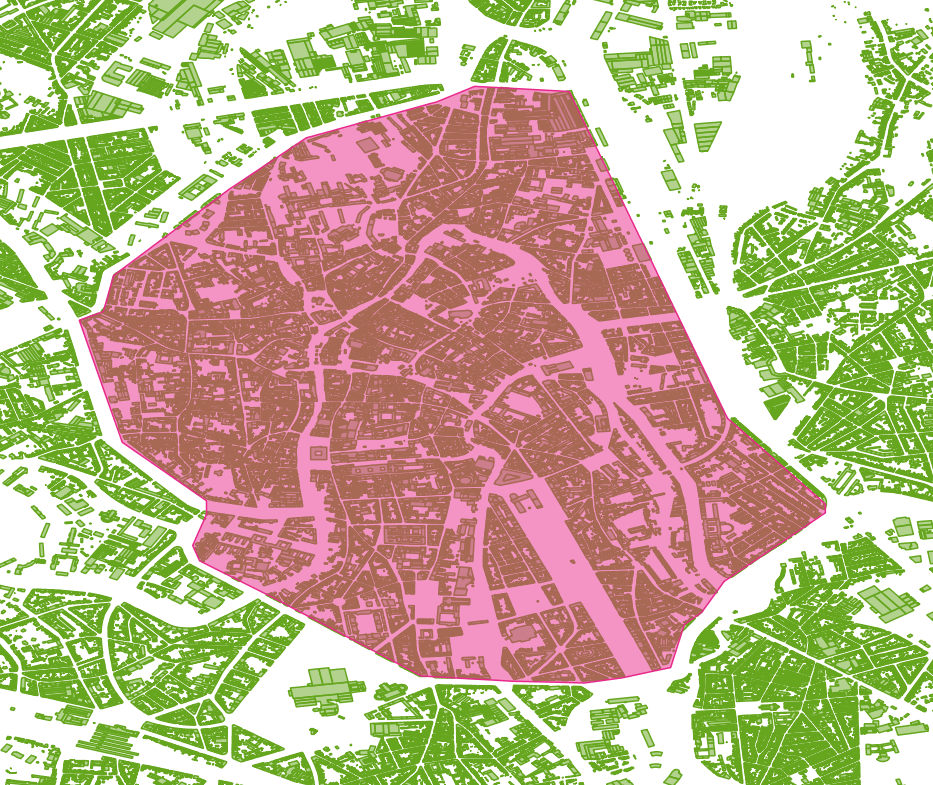
\includegraphics[width=\textwidth]{../images/cityCenterGhent.png}
\caption{The red area covers the city centre of Ghent, Belgium.}
  \label{fig:ghent}
\end{figure}
%%%%%%%%%%%%%%%%%%%%%%%%%%%%%%%%%%%% Scenario 1
\section{Scenario I: A Single User}
\label{sec:scenarios_s1}

This first Scenario will investigate how $SAR_{10g}$ and power consumption behave in an isolated environment meaning there is no influence 
from other base stations or other \gls{UE}. The tool will provision one single drone and position it directly above the user.
Figure \ref{fig:IllustrationS1} illustrates a possible network which satisfies the restrictions of Scenario I. In the middle is the average user drawn with above him the only available \gls{UABS}.
It is clear that the user is only exposed to his own device and the \gls{UABS} above him.
\begin{figure}[H]
\centering
  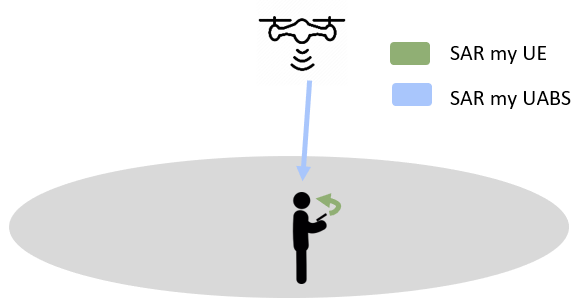
\includegraphics[width=\textwidth/3*2]{../images/IllustrationS1.png}
  \caption{Illustration of an example network that satisfies the restrictions of Scenario I.}
  \label{fig:IllustrationS1}
\end{figure}


These results will however depend on the position of the user. If the randomly generated location of the user is indoor, 
the flying height of the drone might be obstructed by the building where the user resides, causing the user to become uncovered. If this is not the case,
the expected altitude of the user is half of the height of the building meaning that the user would be closer to the \gls{UABS} as 
if he would have been outdoors. Therefore, the user will be positioned outdoor while systematically 
increasing the flying height for more consistent results.

Another considered variable will be the transmission power of the antenna.
\gls{LTE} makes use of power control meaning that no more power will be used than strictly necessary. The actual 
transmission power therefore ranges between zero dBm and the maximum input power. This power is zero when either no user is 
present or the user is so far away that the actual transmitted power would exceed the maximum allowed transmission power.
Increasing the maximum transmission power will not influence the actual power consumption or $SAR_{10g}$ because 
of power control. However, the used transmission power of the \gls{UABS}
does influence power consumption and $SAR_{10g}$ and its behaviour will be investigated at different flying heights.

\begin{wrapfigure}{r}{0.48\textwidth}
  \begin{center}
    \includegraphics[width=0.48\textwidth]{../images/mariahendrikapleinB.png}
  \end{center}
 \caption{Location of `Koningin Maria Hendrikaplein' on the town planning map of Ghent}
  \label{fig:locationHendrikaplein}
\end{wrapfigure}
This scenario investigates $SAR_{10g}$, power consumption and minimal transmission power for two different types of antennae: a 
 fictional \gls{isotropicradiator} and a realistic antenna as presented in table \ref{table:s1:evalpara}.
 The used optimization strategy is not important
for this scenario.
This is because the
 decision algorithm decides which user needs to be connected to which drone. Since only one \gls{UABS} is available,
 both optimization strategies will behave identical. 

The user gets a fixed position. The exact location does not matter as long as it is outside. For this experiment is chosen for the 
`Koningin Maria Hendrikaplein', a square just next to the train station of Ghent (fig. \ref{fig:locationHendrikaplein}).  Doing so will force the \gls{UE} 
to always be at the same height of 1.5 metres. 
An overview of the simulation configuration scenarios is presented in table \ref{table:S1:restrictions}.
\newline
\begin{table}[!htb]
\centering
            \begin{tabular}{|l|l|}
            \hline
            \textbf{Input variables  }                    & \textbf{Output variables}          \\   \hline 
            Type of antenna \{EIRP, microstrip\}            & $SAR_{10g}$  ($W/kg$)            \\ 
            Flying height [20m-200m]                        & Power consumption  ($W$)           \\ 
                                                          &  Minimal $P_{tx}$ ($dBm$)\\ 
                                                          & Electromagnetic field radiation ($V/m$)\\
            \hline
            \end{tabular} 
            \caption{Evaluated parameters}
          \label{table:s1:evalpara}
\end{table}
\begin{table}[!htb]
\centering
        \begin{tabular}{|l|c|l|}
        \hline
        \textbf{Parameter}              & \textbf{Value}          \\   \hline 
        X position user (longitude)              & 3.711198       \\    
        Y position user (latitude)               & 51.036747          \\ 
        Shadow margin             & -3.0398193 \\
        Number of users                & 1 \\
        \hline
        \end{tabular}
        \caption{Restrictions}
        \label{table:S1:restrictions}
\end{table}


Note that there is no explicit restriction on the number of \gls{UAV}s in table \ref{table:S1:restrictions}. The deployment tool initially places 
\gls{UABS}s above each user and it is the optimization strategy that decides which of these potential positions will remain in the end solution.
Since there is only one user, there can also be only one \gls{UAV}.




%%%%%%%%%%%%%%%%%%%%%%%%%%%%%%%%%%%% scenario 2

\FloatBarrier
\section{Scenario II: Increasing Traffic with only one Drone available}

This scenario investigates the same behaviour as the previous one. Still with only one drone but for a higher number of users. 
An illustration of a possible network is given in figure \ref{fig:IllustrationS2}. The average user is drawn in the middle. The only available \gls{UABS} covers him along with the person to the right.
The two other  users at the left side are uncovered and are therefore not  emitting any radiation.
\begin{figure}[H]
\centering
  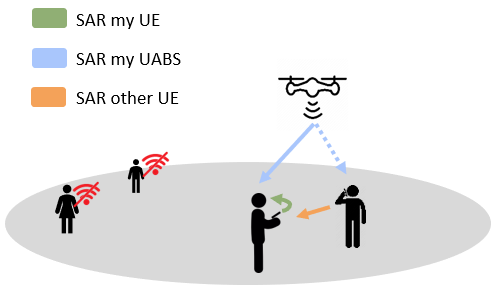
\includegraphics[width=\textwidth/5*3]{../images/IllustrationS2.png}
  \caption{Illustration of an example network that satisfies the restrictions of Scenario II.}
  \label{fig:IllustrationS2}
\end{figure}

Two parameters will be investigated for this scenario. First, the
flying height will be investigated for a fixed number of 224 users. 
This is the number of active users on an average day at 5 p.m. implying rush hour and therefore 
resulting in the highest number of simultaneous users for the day \cite{J2}. The other 
evaluated parameter is a variable number of users. When investigating this 
parameter, the flying height will be fixed to 100 m as recommended by \cite{J2}.
An overview of the evaluated parameters is shown in table \ref{table:s2:evalpara}
 To force the tool to only use one drone, a facility capacity is set to one 
indicating that there is only one spot available in the facility where the \gls{UABS}s are stored. The tool will still consider as much potential places 
as there are users in the network. But when the optimization algorithm is done, only one drone will remain.
On overview of the restrictions is presented in figure \ref{table:S2:restrictions}.

For each parameter investigated, four configurations are possible because there are two antennae available (\gls{isotropicradiator} and a microstrip antenna) which can both operate in a power consumption optimized network or an exposure optimized 
network. The $SAR_{10g}$, power consumption and user coverage will be investigated for all four configurations.

\begin{table}[h]
\centering
            \begin{tabular}{|l|l|}
            \hline
            \textbf{Input variables  }              & \textbf{Output variables}          \\   \hline 
            Type of antenna  \{EIRP, microstrip\}               & $SAR_{10g}$ ($W/kg$)             \\ 
            Flying height [20m-200m]                 & Power consumption ($W$)          \\ 
            Number of users  [50-600]              & User coverage            \\
            Optimization strategy \{Exp Opt, PwrC Opt\}        &     Electromagnetic field radiation ($V/m$)\\
            \hline
            \end{tabular}
            \caption{Evaluated parameters}
          \label{table:s2:evalpara}
\end{table}
\begin{table}[h]
\centering
        \begin{tabular}{|l|c|}
        \hline
        \textbf{Parameter}            & \textbf{Value}       \\   \hline 
        Capacity of the facility          & 1        \\    
        & \\ 
        \hline
        \end{tabular}
        \caption{Restrictions}
        \label{table:S2:restrictions}
\end{table}


%%%%%%%%%%%%%%%%%%%%%%%%%%%%%%%%%%%% scenario 3


\section{Scenario III: Increasing Traffic with an Undefined Amount of Drones}


The third scenario has no restrictions. The tool can use as much \gls{UABS}s as desired while trying to maximize coverage. 
A \gls{UABS} will be considered above each user as was also the case in Scenario II. However, the last step where the capacity of the facility
was checked and drones got eliminated, as discussed in chapter \ref{chap:methodology}, is omitted here. It is expected that the optimization strategies will perform best for this scenario since the decision algorithm has been written
 with multiple drones in mind. 
An illustration is presented in figure \ref{fig:IllustrationS3} with the average user drawn in the middle.
Most users are covered by the many \gls{UABS}s available. The average user 
will be exposed to all these \gls{UABS}s and to all the \gls{UE} that belong to covered users.

\begin{figure}[H]
\centering
  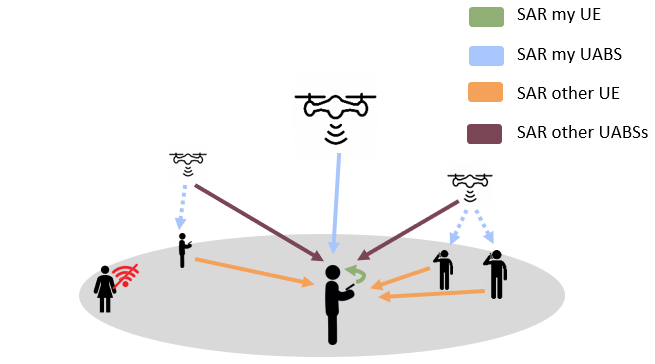
\includegraphics[width=\textwidth/10*7]{../images/IllustrationS3.png}
  \caption{Illustration of an example network according to the description of Scenario III.}
  \label{fig:IllustrationS3}
\end{figure}

Again, two parameters will be evaluated: one with a fixed flying height of 100 m and a variable number of users and a second one with 
a variable flying height and a fixed number of 224 users.
The influence that these input parameters have on the network will be based on the electromagnetic exposure, power consumption, number of drones required and user coverage.
An overview of these parameters is given in table \ref{table:s3:evalpara}.

\begin{table}[!htb]
      \centering
            \begin{tabular}{|l|l|}
            \hline
            \textbf{Input variables  }                        & \textbf{Output variables}       \\   \hline 
            Type of antenna  \{EIRP, microstrip\}               & $SAR_{10g}$ ($W/kg$)                    \\ 
            Flying height    [20-200]                         & Power consumption ($W$)             \\ 
            Number of users  [50-600]                         & User coverage                   \\
            Optimization strategy \{Exp Opt, PwrC Opt\}         &   Electromagnetic field radiation ($V/m$)\\
            \hline
            \end{tabular}
                 \caption{Evaluated parameters}
          \label{table:s3:evalpara}
\end{table}


%%%%%%%%%%%%%%%%%%%%%%%%%%%%%%%%%%%%%%%%%%%%%%%%%%%%%%%%%%%
%\section{Overview of Configurations}
\section{Summary}
Three different scenarios are considered. The first one with single user and a single \gls{UABS}. The second one has 
still only one \gls{UABS} available but has much more users. The third one has an unlimited number of \gls{UABS}s 
available in order to cover as much users as possible.
All three scenarios evaluate the influence of a varying flying height while only the second and third one 
investigate different population sizes.
Four possible configurations exist for each evaluated parameter within each scenario.
The matrix in table \ref{fig:fourCasesMatrix} shows that two types of antennae are investigated.
The microstrip patch antenna and will be abbreviated to microstrip and the \gls{isotropicradiator}
and will be abbreviated as \acs{EIRP}. Both antennae can operate in two 
optimization
strategies: exposure optimized network (\gls{Exp Opt}) and power consumption optimized network (\gls{PwrC Opt}). 
The following chapter reports the results that are achieved from these configurations and scenarios. This will be done by 
monitoring the necessary values during different simulations.

\begin{table}[h!]
\centering
  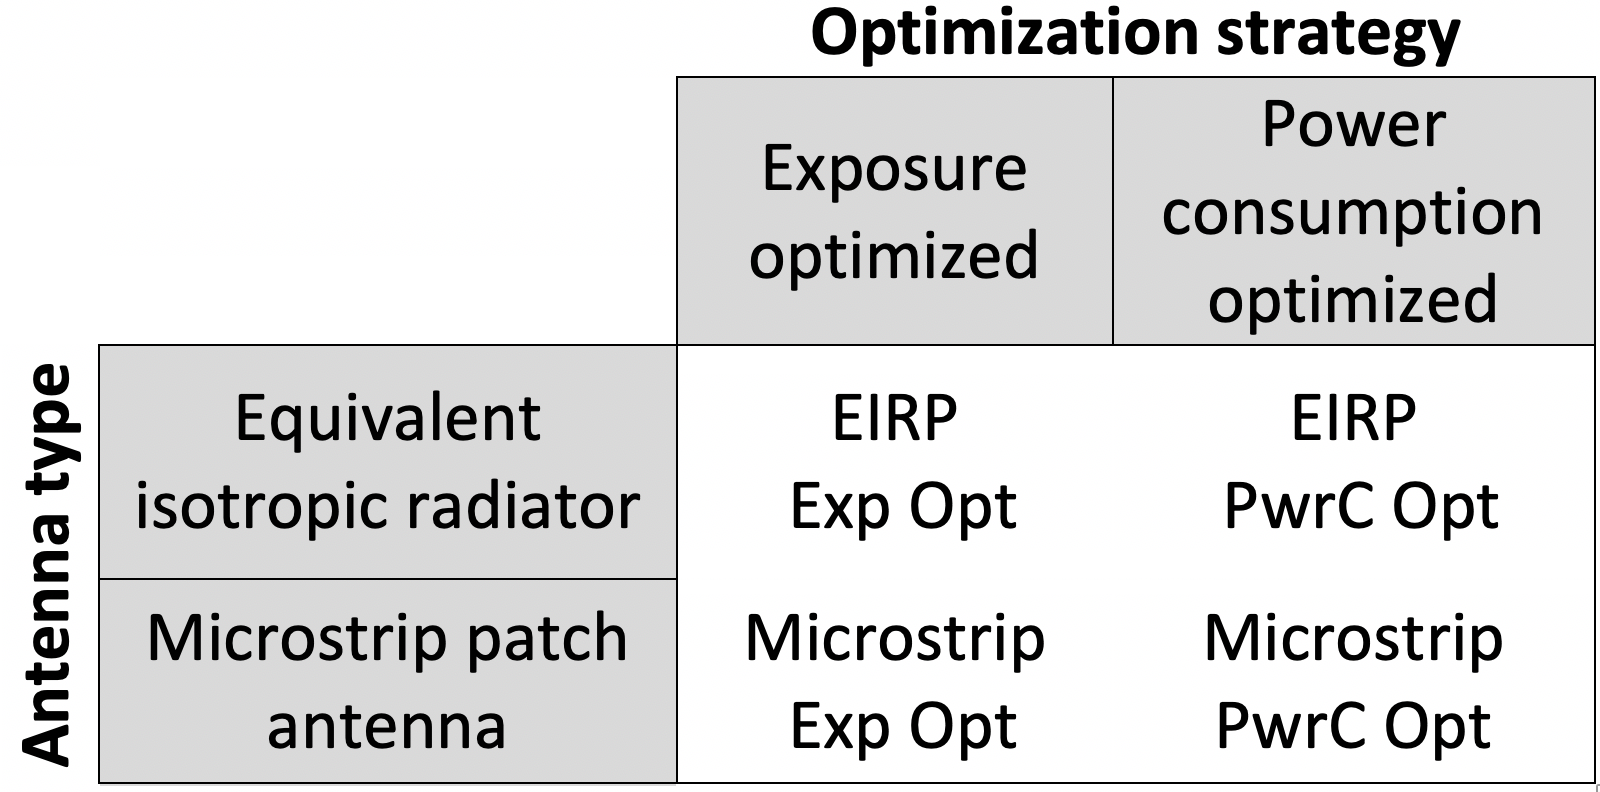
\includegraphics[width=0.8\textwidth]{../images/fourCasesMatrix.png}
  \caption{Matrix with the four possible configurations}
  \label{fig:fourCasesMatrix}
\end{table}




